\documentclass[tikz,border=5pt]{standalone}
\usepackage{pgfplots}
\pgfplotsset{compat=1.18}
\usepackage{fontspec}
\setsansfont{SourceSansPro}[
  Path = /usr/local/texlive/2024/texmf-dist/fonts/opentype/adobe/sourcesanspro/,
  UprightFont = SourceSansPro-Regular.otf,
  BoldFont = SourceSansPro-Bold.otf,
  ItalicFont = SourceSansPro-RegularIt.otf,
  BoldItalicFont = SourceSansPro-BoldIt.otf,
  Scale = 1.0
]
\usetikzlibrary{positioning}
\usepackage{xcolor}
\definecolor{primaryblue}{HTML}{012169}
\definecolor{primarygold}{HTML}{B9975B}
\definecolor{highlightyellow}{HTML}{F2A900}
\definecolor{lightbg}{HTML}{E8EDF5}
\definecolor{jet}{HTML}{1A1A1A}
\definecolor{positivegreen}{HTML}{15803D}
\definecolor{negativered}{HTML}{B91C1C}
\begin{document}
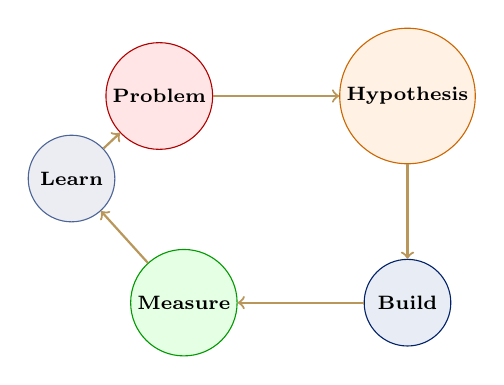
\begin{tikzpicture}[
  node distance=1.2cm and 1.6cm,
  cnode/.style={draw, circle, minimum size=1.1cm, font=\scriptsize\bfseries,
                align=center, inner sep=2pt},
  arr/.style={->, thick, color=primarygold}
]
  \node[cnode, draw=red!70!black,    fill=red!10]     (P) {Problem};
  \node[cnode, draw=orange!80!black, fill=orange!10,  right=of P] (H) {Hypothesis};
  \node[cnode, draw=primaryblue,     fill=lightbg,    below=of H] (B) {Build};
  \node[cnode, draw=green!60!black,  fill=green!10,   left=of B]  (M) {Measure};
  \node[cnode, draw=primaryblue!70,  fill=primaryblue!8, above left=0.7cm and 0.55cm of M] (L) {Learn};

  \draw[arr] (P) -- (H);
  \draw[arr] (H) -- (B);
  \draw[arr] (B) -- (M);
  \draw[arr] (M) -- (L);
  \draw[arr] (L) -- (P);
\end{tikzpicture}
\end{document}
